\section{\OSname{} 多核调度器设计}
\label{sec:design-overview}
% The \OSname{} scheduler is tickless and implements a preemptive priority scheduling policy that always executes the highest priority thread.
% For multicore, this policy is abstracted so that the scheduler must execute the \textit{n} highest priority threads on the \textit{n} available cores.
% In the following, without loss of generality, we assume $N=2$ cores (Core 0 and Core 1). Note, however, that scaling to $N>2$ is trivial, assuming $N$ and $n$ remain small as per our goals (recall~\autoref{sec:goals}).
在下文中,不失一般性,我们假设 $N=2$ 个核心(核心 0 和核心 1)。然而,需要注意的是,扩展到 $N>2$ 是微不足道的,前提是 $N$ 和 $n$ 保持较小,符合我们的目标(回顾~\autoref{sec:goals})。

% \subsection{Startup}

% The \OSname{} runtime initialization executes on Core 0, while the other core is in deep sleep or stall mode. 
% % \paragraph*{Starting Secondary Cores} 
% After the general initialization on Core 0, Core 1 is set up with the shared interrupt vector table (IVT), a separate main stack pointer (SP), and an entry function that, down the line, will start threading on this core, analogous to Core 0.
% This is depicted in Fig.~\ref{fig:startup}.
% Threading is started by enabling the scheduler interrupt at the lowest priority and invoking the scheduler, which will then select the next thread for the core.
\subsection{启动}

\OSname{} 操作系统运行时初始化在核心0上执行,而另一个核心则处于深度休眠或停滞模式。
在核心 0 上完成通用初始化后,核心 1 将设置使用共享中断向量表(IVT)、一个独立的主栈指针(SP),以及一个入口函数,该函数最终将在该核心上启动线程,类似于核心 0。
这一过程如图~\ref{fig:startup} 所示。
线程启动是通过启用最低优先级的调度中断并调用调度器来实现的,调度器随后会选择下一个线程进入核心。

%\begin{itemize}
%    \item Insert figure figures/startup.png?
%\end{itemize}

% \noteEB{in Fig. 1 comes through as though Core 0 does not make use of a stack pointer, vector table etc. Is this wanted?}
% \noteEF{Agree that it is a bit unclear. The graph was from the perspective of the threading module, i.e. "what happens when \textit{start\_threading} is called". I included stack pointer, entry function and vector table because they are transferred from core 0 to core 1. I added a version figures/startup-2.png that also includes them for core 0. But I'm not sure if it look weird having them just "floating around" there.}


\begin{figure}
\iffalse
\footnotesize
    \begin{tikzpicture}  
        \tikzset{>=stealth}  
        \tikzstyle{arr} = [thick],  
        \tikzstyle{process} = [shape=rectangle, rounded corners, align=center, draw, minimum width=2.5cm, fill=white],  
        \tikzstyle{data} = [shape=circle, align=center, draw, minimum width=1cm, fill=white],  
        \coordinate (bottomend) at (\columnwidth, 0);  
        \coordinate (bottombegin) at (0, 0);  
        \coordinate (bottommid) at ($(bottomend)!0.5!(bottombegin)$);  
        \coordinate (core0end) at ($(bottommid) - (0.25, 0)$);  
        \coordinate (core1start) at ($(bottommid) + (0.25, 0)$);  
        \coordinate (core0mid) at ($(core0end)!0.5!(bottombegin)$);  
        \coordinate (core1mid) at ($(core1start)!0.5!(bottomend)$);  
   
        \node [process, anchor=south, name=schedule] at (0,0.25 -| core0mid) {Schedule};  
        \node [process, anchor=south, name=irq, yshift=0.25cm] at (schedule.north) {Enable Scheduler\\Interrupt};  
        \node [process, anchor=south, name=otherCore, yshift=0.25cm] at (irq.north) {Start up Other\\Core};  
        \node [process, anchor=south, name=idle, yshift=0.25cm] at (otherCore.north) {Create Idle\\Threads};  
   
        \node [data, anchor=south, name=ef0, yshift=0.25cm] at (idle.north) {Entry\\Point};  
        % \node [data, anchor=south, name=vt0] at ($(ef0.north -| bottombegin)!0.5!(ef0.north)$) {IVT};  
        \node [data, name=vt0, xshift=-0.5cm] at (ef0.west) {IVT};  
        % \node [data, anchor=south, name=sp0] at ($(ef0.north)!0.5!(ef0.north -| core0end)$) {SP};  
        \node [data, name=sp0, xshift=0.5cm] at (ef0.east) {SP};  
  
        % core 1  
        \node [process, anchor=south, name=schedule1] at (0,0.25 -| core1mid) {Schedule};  
        \node [process, anchor=south, name=irq1, yshift=0.25cm] at (schedule1.north) {Enable Scheduler\\Interrupt};  
  
        \node [data, anchor=south, name=ef1, yshift=0.25cm] at (irq1.north) {Entry\\Point};  
        % \node [data, anchor=south, name=vt1] at ($(ef1.north -| core1start)!0.5!(ef1.north)$) {IVT};  
        % \node [data, anchor=south, name=sp1] at ($(ef1.north)!0.5!(ef1.north -| bottomend)$) {SP}; 
        \node [data, name=vt1, xshift=-0.5cm] at (ef1.west) {IVT}; 
        \node [data, name=sp1, xshift=0.5cm] at (ef1.east) {SP};  
        \draw [dashed] (vt1.west |- vt1.north) rectangle (sp1.east |- ef1.south);   
  
        % arrows  
        \draw [arr,->] (ef0.south) -- (idle.north);  
        \draw [arr,->] (idle.south) -- (otherCore.north);  
        \draw [arr,->] (otherCore.south) -- (irq.north);  
        \draw [arr,->] (irq.south) -- (schedule.north);  
  
        \draw [arr,->] (irq1.south) -- (schedule1.north);  
        \draw [arr,->] (ef1.south) -- (irq1.north);  
        
  
        \draw [thick, double distance=0.5cm, {-Triangle[scale=0.5,fill=white]}] (otherCore.east) -- (vt1.west |- otherCore.east);  
                                                                                      
        \coordinate (topend) at ($(\columnwidth,0 |- sp0.north) + (0,0.75)$);         
        \coordinate (topbegin) at (0, 0 |- topend);                                   
        \coordinate (topmid) at ($(topend)!0.5!(topbegin)$);                          
        \coordinate (core0northeast) at ($(topmid) - (0.25, 0)$);                     
        \coordinate (core1northwest) at ($(topmid) + (0.25, 0)$);                     
                                                                                      
        \node [anchor=north west, xshift=10pt, yshift=-5pt] at (topbegin) {\texttt{Core 0}};       
        \node [anchor=north west, xshift=10pt, yshift=-5pt] at (core1northwest) {\texttt{Core 1}};  
        \begin{scope}[on background layer]                                            
            \draw [rounded corners=15pt, fill=gray!10] (topend |- 0,0) rectangle (core1northwest);  
            \draw [rounded corners=15pt] (0, 0) rectangle (core0northeast);           
            \draw [fill=gray!10, draw=gray!10] ($(idle.north -| bottombegin) + (0.25,0.15)$) rectangle ($(otherCore.south -| core0end) - (0.25,0.15)$);  
        \end{scope}                                                                   
                                                                                      
    \end{tikzpicture}                                

\fi
\centering
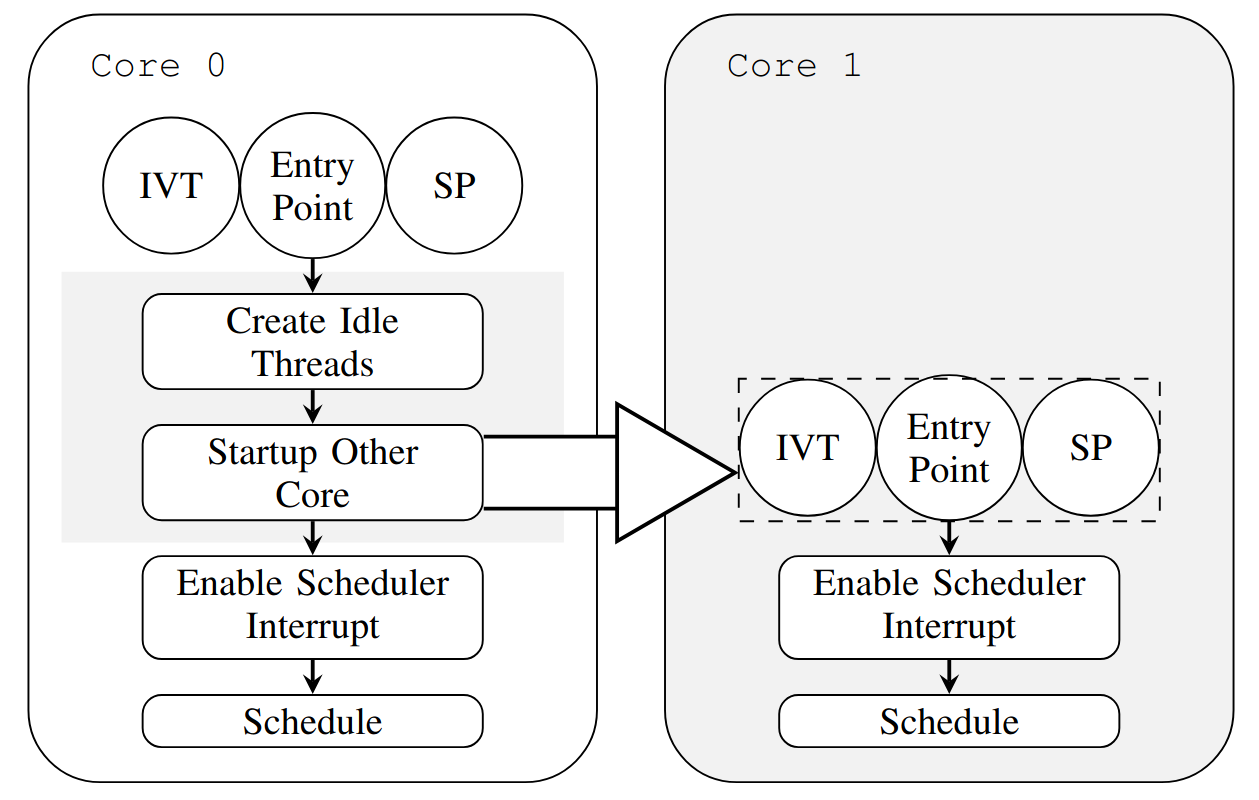
\includegraphics[width=0.95\columnwidth]{translate/figures/threading-startup-render-2.png}
     \caption{双核系统上的线程启动}
     \label{fig:startup}
 \end{figure}




\iffalse
\subsection{Idle Threads}

When a core is idle, it is prompted to enter low-power mode until the next thread is ready and waiting.
% Two alternative mechanisms are used to enter idle mode, depending on whether a system is single- or multicore. %\noteCA{``Two'' mechanisms?} 
On single-core, idle mode is entered in the scheduler exception, resulting in a lazy context switch (i.e. context is switched only when a different thread requires that). 
On multicore, however, such lazy context switching can result in race conditions, and thus idle threads are used instead.
% More in details: one idle thread is created per core during startup at the lowest priority.
% When no other thread is ready, the scheduler will execute this thread.
The idle threads execute at lowest priority and simply prompt the core to enter low-power mode until an interrupt occurs.
\fi

\subsection{全局调度方案}\label{sec:design:scheduling}


% \begin{itemize}
%     \item Two alternative designs: \textit{Global reallocation} routine (ThreadX) and \textit{Dynamic selection} (FreeRTOS, Nuttx, RT-Thread) approach
%     \begin{itemize}
%         \item 2-3 sentences each how they work on a high level
%     \end{itemize}
% \end{itemize}



% \OSname{} uses a global scheduling scheme.

% Global scheduling facilitates thread migration, where threads migrate between cores between executions.
% We chose global scheduling because it reduces context switches and priority inversions, and makes better use of the overall capacity~\cite{hardrealtime-multiprocessor-survey, brandenburg}.
% Furthermore, it avoids the thread allocation problem of partitioned scheduling, i.e., the problem of finding an optimal allocation of threads to cores.
% The main drawback of global scheduling is scalability, when the global runqueue becomes a bottleneck for context switching~\cite{EDF-RM-multiprocessor-survey}. However, this issue is negligible on MCUs --- which have a low processor count.
\OSname{} 使用全局调度方案

全局调度支持线程迁移,允许线程在执行过程中在不同核心之间动态移动。我们选择全局调度,是因为它能够有效减少上下文切换的频率,降低优先级反转的风险,并且更高效地利用整体计算资源~\cite{hardrealtime-multiprocessor-survey, brandenburg}。此外,全局调度还避免了分区调度中常见的线程分配难题,即如何为每个核心找到最优的线程分配方案。全局调度的主要缺点是其在可扩展性方面的局限性,尤其是在全局运行队列可能成为上下文切换瓶颈的情况下~\cite{EDF-RM-multiprocessor-survey}。然而,在微控制器场景中,由于处理器核心数量通常较少,这一问题的影响几乎可以忽略不计。


% \subsection{Assigning Threads to Cores}
% \label{sec:Assigning-Threads-to-Cores}
% With the single-core configuration, the thread-selection process simply reads the head of the runqueue. 
% However, on multicore, this would result in the same thread being executed on multiple cores.
% There are various approaches for selecting the next thread that a core should execute.
% We initially designed our scheduler so that it can accommodate either \textit{core reallocation} or alternatively \textit{dynamic thread selection} (see \autoref{sec:multicore-sched}). We then implemented both, before reporting on their performance on different hardware in \autoref{sec:benchmarks}.
\subsection{线程分配到核}
\label{sec:Assigning-Threads-to-Cores}
在单核配置中,线程选择过程仅需读取运行队列的头部。然而,在多核配置下,这种简单的选择方式会导致同一个线程在多个核上被执行。为了避免这种情况,我们探索了多种线程分配策略。我们最初设计的调度器能够灵活支持 \textit{核重分配} 或 \textit{动态线程选择}(参见 \autoref{sec:multicore-sched})。此后,我们不仅实现了这两种方法,还在 \autoref{sec:benchmarks} 中详细报告了它们在不同硬件平台上的性能表现。
%in our multicore effort in order to make an informed decision for our final implementation.

%  \begin{figure}[b]
%      \centering
%      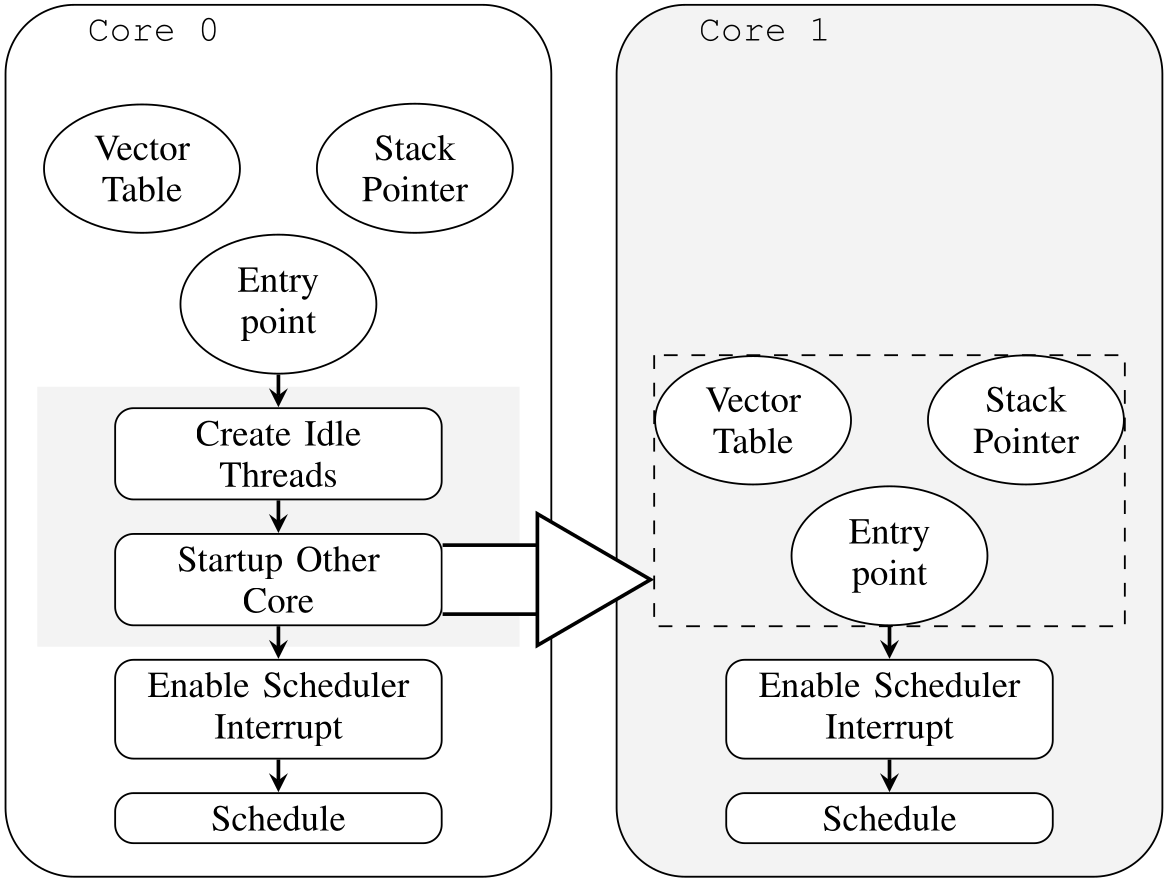
\includegraphics[width=\linewidth]{figures/threading-startup-render.png}
%      \caption{Threading startup on a dual-core system.}
%      \label{fig:startup}
%  \end{figure}

\iffalse
\subsubsection{Core Reallocation}

With this approach, a \textit{reallocation} routine maps the \textit{n} highest priority threads to the \textit{n} cores.
The allocation for each core is stored in an array that the scheduler interrupt handler reads upon invocation.
After each change in the runqueue, the \textit{reallocation} routine is executed.
It compares the previous allocation with the current highest priority threads in the runqueue, and updates the core allocation list with the goal of minimizing changes, and thus thread migration.
Based on the allocation changes, the routine returns the ID of the core where a context switch is needed.
A prominent example that follows this design is the ThreadX operating system.

\subsubsection{Dynamic Thread Selection}

In an alternative approach, implemented in FreeRTOS, NuttX, Zephyr or RT-Thread, the next thread for a core is selected directly from the runqueue by the scheduler interrupt handler upon invocation.
The thread is then removed from the runqueue to prevent it from being selected for multiple cores.
Conversely, when a running thread is preempted, it is re-added to the runqueue.
The scheduler uses the information it has readily available about thread state changes to trigger a scheduler interrupt on the specific core where a context switch is needed.
For instance, if a high-priority thread becomes ready, the scheduler interrupt is set for the core that is currently executing the lowest-priority thread.

\fi

% In an alternative approach, the scheduler selects the next thread for a core, in a dynamic fashion, upon invocation.
% The global scheduler uses the information it has readily available about changes in thread state changes, in the runqueue changes, to invoke the scheduler on the specific core where a context switch is needed.
% \noteEB{I attempted reformulation because it was difficult to parse. But somehow it is *still* difficult to parse. In particular, if there is a global scheduler, it should not sound suddenly like there are multiple schedulers...}
% The scheduler then %reads the next thread from the runqueue and 
% removes the thread from the runqueue, to prevent the same thread from being selected for multiple cores.
% Conversely, when a running thread is preempted, it is re-added to the runqueue.
% \subsection{Core Affinity Masks}

% Core affinities are a feature that allows pinning a thread so it runs on some specified core(s) only. %one or multiple specific cores. 
% This provides the user with fine-grained control over how and where threads may run. 
% % For example, core affinities can be used to bind two threads with different priorities to the same core, which will ensure that they can not run in parallel, and thus mutual exclusion between them.
% Core affinities are realized with a bitmask, where a set bit encodes that the thread can run on the core with this index. 
% The scheduler uses this information when selecting the core on which a thread should run.

\subsection{核亲和性掩码}

核亲和性是一种特性,允许将线程固定到特定的核上运行。这为用户提供了对线程运行位置和方式的精细控制。

核亲和性通过位掩码实现,其中设置的位表示线程可以在该索引对应的核上运行。调度器在选择线程应运行的核时会使用这些信息

% \subsection{Dynamic Priorities and Priority Inheritance}

% Thread priorities in \OSname{} can be changed dynamically at runtime for all active threads.
% A change in priority may result in a context switch if a running thread's priority is decreased or if a waiting thread's one increased.
% Furthermore, dynamic priorities facilitate priority inheritance for mutexes.
% If a higher-priority thread is blocked on a mutex that is currently owned by a lower-priority thread, the owning thread inherits the higher priority of the waiting thread.
% This prevents the owner from being preempted by other lower-priority threads 
% and thus helps avoid priority inversions caused by indirect blocking.

\subsection{动态优先级与优先级继承}

在 \OSname{} 中,所有活动线程的优先级都可以在运行时动态调整。如果运行中的线程优先级被降低,或者等待中的线程优先级被提高,这可能会触发上下文切换。此外,动态优先级还支持互斥锁的优先级继承。当一个高优先级线程因等待一个当前由低优先级线程持有的互斥锁而阻塞时,持有互斥锁的线程将继承等待线程的较高优先级。这可以防止持有者被其他低优先级线程抢占,从而有助于避免由间接阻塞引起的优先级反转问题。

% \subsection{Synchronization in the Scheduler\label{sec:design:sync}}

% \OSname{} implements mutual exclusion in the kernel through a global critical section, effectively resulting in a \textit{Big Lock} design.
% Thus, there is no concurrency in the kernel, which is tolerable given that such operations in \OSname{} are short.
% It ensures correctness, prevents data races and deadlocks, and simplifies operations that involve multiple data structures, such as the runqueue and Thread Control Blocks (TCBs), because no individual locking is needed.
% On single-core systems, it is sufficient to mask all interrupts to create a critical section.
% In multicore systems, an additional global spinlock is required to ensure that even threads on other cores cannot enter another critical section. 

\subsection{调度器中的同步\label{sec:design:sync}}

\OSname{} 通过全局临界区在内核中实现互斥,这实际上形成了一种 \textit{大锁} 设计。
因此,在内核中不存在并发问题,鉴于 \OSname{} 中此类操作的持续时间较短,这种设计是可以接受的。
它确保了操作的正确性,防止了数据竞争和死锁,并且简化了涉及多个数据结构的操作,例如运行队列和线程控制块(TCBs),因为无需单独锁定。
在单核系统中,屏蔽所有中断就足以创建一个临界区。
在多核系统中,需要额外的全局自旋锁来确保其他核心上的线程也无法进入另一个临界区。

% \subsection{Combining Scheduled Threads \& Async Rust Tasks}\label{sec:design:async}

% \OSname{} uses async code based on \emph{Embassy}~\cite{embassy} for system initialization and in the HAL.  
% There is always a system executor for async tasks. 
% Using the preemptive scheduler --- and thus threading --- is optional. 
% If the scheduler is not used, the system executor will run in interrupt context. 
% If the scheduler is used, the system executor executes in a thread. 
% Additional executors can be started in other threads. 
% When all tasks on an executor are pending, the owning thread is suspended. 
% Threads can block on async functions and wait for async resources from an executor.
% Thus, the gap is bridged between the scheduler, async Rust, future-based concurrency, and asynchronous I/O.

\subsection{调度线程与异步 Rust 任务结合}\label{sec:design:async}

\OSname{} 使用基于 \emph{Embassy}~\cite{embassy} 的异步代码进行系统初始化和硬件抽象层(HAL)的实现。
系统中始终存在一个用于执行异步任务的系统执行器.
使用抢占式调度器以及由此产生的线程是可选的。如果未使用调度器,系统执行器将在中断上下文中运行。如果使用了调度器,系统执行器则会在一个线程中执行。额外的执行器可以在其他线程中启动。当某个执行器上的所有任务都处于挂起状态时,拥有该执行器的线程将被挂起。线程可以阻塞在异步函数上,并等待来自执行器的异步资源。
因此,\OSname{} 在调度器、异步Rust、基于future的并发以及异步I/O之间架起了桥梁。




% 
% DRAFT THAT FIRST: Goals (and non-goals) in conjunction with benchmarks planned
% (with starting point: single-core scheduler is like RIOT-rs scheduler)


% - discussion of scheduler variants:
%    - mentioned that we face crossroad/ two avenues; shortly discuss them
%    - we tested them on two platforms; compare in one benchmark, max two
%    - reduced
%    - "present thesis in two minutes"
%    - describe all feature